\section{Ứng dụng đạo hàm để giải quyết một số vấn đề liên quan đến thực tiễn}
\subsection{Đề 1}
\Opensolutionfile{ans}[ans/ans-0-B5]
\caulc
\begin{ex}%[2D1H3-6]
	Một chất điểm chuyển động theo quy luật $s(t) = t^2 - \dfrac{1}{6}t^3$ (m). Tìm thời điểm $t$ (giây) mà tại đó tốc độ $v$ (m/s) của chuyển động đạt giá trị lớn nhất.
	\choice
	{$t = 2{,}5$}
	{$t = 1$}
	{\True $t = 2$}
	{$t = 0{,}5$}
	\loigiai{
		Ta có $v(t) = s'(t) = 2t - \dfrac{1}{2}t^2$.\\
		Suy ra $v'(t) = 2 - t$ và $v'(t) = 0 \Leftrightarrow t = 2$.\\
		Bảng biến thiên
		\begin{center}
			
\begin{tikzpicture}
				\tkzTabInit[lgt=1.2,espcl=4]
				{$t$/1,$v’(t)$/1,$v(t)$/2}
				{$0$,$2$,$+\infty$}
				\tkzTabLine{ ,+,0,-, }
				\tkzTabVar{-/,+/$2$,-/}
			\end{tikzpicture}
		\end{center}
		Vậy chất điểm đạt tốc độ lớn nhất tại thời điểm $t = 2$ (giây).
	}
\end{ex}

\begin{ex}%[2D1H3-6]
	Một vật chuyển động theo quy luật $s=\dfrac{1}{3}t^3-t^2+9t$ với $t$ (giây) là khoảng thời gian tính từ lúc vật bắt đầu chuyển động và $s$ (mét) là quãng đường đi được trong thời gian đó. Hỏi trong khoảng thời gian $10$ giây kể từ lúc bắt đầu chuyển động, tốc độ lớn nhất của vật đạt được bằng bao nhiêu?
	\choice
	{$109\left(\mathrm{m/s}\right)$}
	{\True $89\left(\mathrm{m/s}\right)$}
	{$\dfrac{25}{3}\left(\mathrm{m/s}\right)$}
	{$71\left(\mathrm{m/s}\right)$}
	\loigiai{
		Vì $s(t)=\dfrac{1}{3}t^3-t^2+9t\Rightarrow v(t)=t^2-2t+9$.\\
		Xét hàm $f(t)=t^2-2t+9\Rightarrow f'(t)=2t-2=0\Rightarrow t=1$.\\
		Bảng biến thiên của hàm số $f(t)=t^2-2t+9$ với $0<t\leq 10$.
		\begin{center}
			
\begin{tikzpicture}
				\tkzTabInit[nocadre,lgt=1.2,espcl=3.5]{$t$/0.7,$f'(t)$/0.7,$f(t)$/2.5}{$0$,$1$,$10$}
				\tkzTabLine{,{},0,{},}
				\tkzTabVar{+/$9$,-/$8$,+/$89$}
			\end{tikzpicture}
		\end{center}
		Dựa vào bảng biến thiên ta thấy tốc độ của vật đạt được lớn nhất bằng $89$ (m/s).
	}
\end{ex}


\begin{ex}%[2D1H3-6]
	Trong một môi trường dinh dưỡng có  $1\,000$  vi khuẩn được cấy vào. Bằng thực nghiệm xác định được số lượng vi khuẩn tăng theo thời gian bởi quy luật $N(t)=1\,000+\dfrac{100t}{100+t^2}$ (con vi khuẩn), trong đó $t$ là thời gian (đơn vị giây). Hãy xác định thời điểm sau khi thực hiện cấy vi khuẩn vào, số lượng vi khuẩn tăng lên lớn nhất? 
	\choice
	{$0$}
	{$1$}
	{$-10$}
	{\True $10$}
	\loigiai{
		Ta có tốc độ phát triển của đàn vi khuẩn tại thời điểm $t$ là\\
		$$
		N'(t)=\dfrac{100\left(100+t^2\right)-100t(2t)}{\left(100+t^2\right)}=\dfrac{100^2-100t^2}{\left(100+t^2\right)^2} \, (\forall t>0).
		$$
		Xét $N'(t)=0 \Leftrightarrow t^2=100 \Leftrightarrow \hoac{&t=-10 \quad \text{(loại)} \\ & t=10 \quad \text{(nhận).}}$\\
		Lập bảng biến thiên ta được
		\begin{center}
		
\begin{tikzpicture}[scale=1, font=\footnotesize, line join=round, line cap=round, >=stealth]
			\tkzTabInit[nocadre=false,lgt=1.5,espcl=2,deltacl=0.5]
			{$t$/.7 ,$N'(t)$/.7,$N(t)$/2}
			{$0$ , $10$ , $+\infty$}
			\tkzTabLine{ , + , $0$ , - , }
			\tkzTabVar{-/, +/$1005$ , -/}
		\end{tikzpicture}
		\end{center}
	Dựa vào bảng biến thiên, ta kết luận số lượng vi khuẩn tăng lên lớn nhất tại thời điểm $t=10$.
	}
\end{ex}



\begin{ex}%[2D1H3-6]
	Mỗi đợt xuất khẩu gạo của tỉnh A thường kéo dài trong $60$ ngày. Người ta nhận thấy lượng gạo xuất khẩu tính theo ngày thứ $t$ được xác định bởi công thức: $S(t)=\dfrac{2}{5}t^3-63t^2+3240t-3100$ (tấn) $(1 \le t \le 60)$. Hỏi trong $60$ ngày đó, ngày thứ mấy có lượng gạo xuất khẩu cao nhất?
	\choice
	{$60$}
	{\True $45$}
	{$30$}
	{$25$}
	\loigiai{Xét hàm số $S(t)=\dfrac{2}{5}t^3-63t^2+3\,240t-3\,100$ với $t \in [1;60]$.\\
		Ta có $S'(t)=\dfrac{6}{5}t^2-126t+3240$.\\
		\hspace*{1cm} $S'(t)=0 \Leftrightarrow \hoac{&t=45 \\ &t=60.}$\\
		Vì $S(1)=\dfrac{387}{5}$, $S(45)=51\,575$, $S(60)=50\,900$ nên ta được $\max \limits_{t \in [1;60]} S(t)=S(45)=51\,575$.\\
		Vậy ngày thứ $45$ là ngày có lượng gạo xuất khẩu cao nhất.}
\end{ex}


\begin{ex}%[2D1H3-6]
	Trong các hình chữ nhật có chu vi là $24$ cm, hãy tìm hình chữ nhật có diện tích lớn nhất. 
	\choice
	{\True $36$}
	{$24$}
	{$48$}
	{$72$}
	\loigiai{
		Gọi $x$ (cm) là chiều rộng của hình chữ nhật.\\
		Điều kiện $0<x<12$.\\
		Chiều dài của hình chữ nhật là $12-x$ (cm).\\
		Diện tích của hình chữ nhật là $x(12-x)=-x^2+12x$ (cm$^2$).\\
		Xét hàm số $y=-x^2+12x$ với $0<x<12$.\\
		Ta có $y'=-2x+12$; $y'=0 \Leftrightarrow x=6$.
		$$
		y(0)=0;\,y(6)=36;\,y(12)=0.
		$$
		Do đó $\max\limits_{(0;12)} y=y(6)=36$.\\
		Trong các hình chữ nhật có chu vi là $24$ (cm) thì hình vuông có diện tích lớn nhất.
	}
\end{ex}



\begin{ex}%[2D1H2-7] 
	Độ giảm huyết áp của một bệnh $G(x)=0{,}025x^2(30-x)$ trong đó $x$ là số miligam thuốc được tiêm cho bệnh nhân $(0<x<30)$. Để bệnh nhân đó có huyết áp giảm nhiều nhất thì liều lượng thuốc cần tiêm vào là 
	\choice
	{$x=15$ (mg)}
	{$x=20$ (mg)}
	{\True  $x=20$ (mg)}
	{$x=25$ (mg)}
	\loigiai{
	$G'(x)=1{,}5x-0,075x^2 
	\Rightarrow G'(x)=0 \Leftrightarrow \hoac{&x=0\\&x=20.}$\\
	Bảng biến thiên 
	\begin{center}
		
\begin{tikzpicture}[scale=1, font=\footnotesize, line join=round, line cap=round, >=stealth]
		\tkzTabInit[nocadre=false,lgt=1.5,espcl=2,deltacl=0.5]
		{$x$/.7 ,$G'(x)$/.7,$G(x)$/2}
		{$0$ , $20$ , $30$}
		\tkzTabLine{ , + , $0$ , - , }
		\tkzTabVar{-/$0$ , +/$100$ , -/$0$}
	\end{tikzpicture}
	\end{center}
	Vậy để bệnh nhân đó có huyết áp giảm nhiều nhất thì liều lượng thuốc cần tiêm vào là $x=20$ (mg).
	}
\end{ex}


\begin{ex}%[2D1H1-5]
	Sự ảnh hưởng khi sử dụng một loại độc tố với vi khuẩn $X$ được một nhà sinh học mô tả bởi hàm số $P(t)=\dfrac{t+1}{t^2+t+4}$, trong đó $P(t)$ là số lượng vi khuẩn sau $t$ giờ sử dụng độc tố. Vào thời điểm nào thì số lượng vi khuẩn $X$ bắt đầu giảm? 
	\choice
	{Ngay từ lúc bắt đầu sử dụng độc tố}
	{Sau $0{,}5$ giờ}
	{Sau $2$ giờ}
	{\True  Sau $1$ giờ}
	\loigiai{
	Ta có $P'(t)=\dfrac{-t^2-2t+3}{\left(t^2+t+4\right)^2}=\dfrac{(t-1)(-t-3)}{\left(t^2+t+4\right)^2} \quad (t>0)$.\\
	$\Rightarrow 	P'(t)=0 \Leftrightarrow \hoac{&t=-3 \quad \text{(loại)}\\&t=1 \quad \text{(nhận)}.}$\\
	Bảng biến thiên 
	\begin{center}
	
\begin{tikzpicture}[scale=1, font=\footnotesize, line join=round, line cap=round, >=stealth]
		\tkzTabInit[nocadre=false,lgt=1.5,espcl=2,deltacl=0.5]
		{$t$/.7 ,$P'(t)$/.7,$P(t)$/2}
		{$0$ , $1$ , $+\infty$}
		\tkzTabLine{ , + , $0$ , - , }
		\tkzTabVar{-/$\dfrac{1}{4}$ , +/$\dfrac{1}{3}$ , -/$0$}
	\end{tikzpicture}
	\end{center}
	Ta thấy hàm số đạt cực đại tại $t=1$ và $P'(t)<0, \forall t \in(1;+\infty)$ nên sau $1$ giờ thì vi khuẩn bắt đầu giảm.
	}
\end{ex}

\begin{ex}%[2D1V3-6]
	\immini{
	Một người thợ gò làm một cái hòm dạng hình hộp chữ nhật có nắp bằng tôn. Biết rằng độ dài đường chéo hình hộp bằng $3\sqrt{2}$ dm và chỉ được sử dụng vừa đủ $18$ dm$^2$ tôn. Với yêu cầu như trên người thợ có thể làm được cái hòm có thể tích lớn nhất bằng 
	\choice
	{$8$ dm$^3$}
	{$2 \sqrt{2}$ dm$^3$}
	{$6$ dm$^3$}
	{\True  $4$ dm$^3$}}{
	\begin{tikzpicture}[scale=.8, font=\footnotesize, line join=round, line cap=round, >=stealth]
	\def\a{5}
	\def\b{2}
	\def\h{2}
	\path 	(0:0) coordinate (A)
			++(0:\a) coordinate (D)
			++(-130:\b) coordinate (C)
			($(A)+(C)-(D)$) coordinate (B)
			($(A)+(90:\h)$) coordinate (A')
			($(B)+(90:\h)$) coordinate (B')
			($(C)+(90:\h)$) coordinate (C')
			($(D)+(90:\h)$) coordinate (D');
	\draw[dashed,thick] 	(B)--(A)--(D)	(A)--(A');
	\draw[thick] 	(C)--(C') 	(D)--(D') 	(B)--(B')	(C)--(C')
			(B)--(C)--(D) 
			(A')--(B')--(C')--(D')--cycle;
	\end{tikzpicture}
	}
	\loigiai{
		Gọi $a$, $b$, $c$ ($a>0$, $b>0$, $c>0$) là  $3$  kích thước của hình hộp chữ nhật. Không mất tính tổng quát, giả sử $0<c \leq b \leq a$.\\
		Theo giả thiết $\sqrt{a^2+b^2+c^2}=3 \sqrt{2} \Rightarrow a^2+b^2+c^2=18. \quad (1)$\\
		Diện tích toàn phần của khối hộp là $2a b+2b c+2c a=18. \quad(2)$\\
		Từ $(1)$, $(2)$ ta có $(a+b+c)^2=a^2+b^2+c^2+2a b+2b c+2c a=36 \Rightarrow a+b+c=6. \quad (3)$\\
		Từ $(3)$, $(2)$ ta có $a b+c(6-c)=9 \Rightarrow a b=9+c^2-6c$.\\
		Thể tích của cái hòm $V=a b c=\left(c^2-6c+9\right) c=c^3-6c^2+9c, \,(0<c<\sqrt{6})$.\\
		Đặt $h(c)=c^3-6c^2+9c \Rightarrow h'(c)=3c^2-12c+9 \Rightarrow h'(c)=0 \Leftrightarrow \hoac{&c=1 \quad \text{(nhận)}\\& c=3 \quad \text{(loại)}.}$\\
		Bảng biến thiên
		\begin{center}
		
\begin{tikzpicture}[scale=1, font=\footnotesize, line join=round, line cap=round, >=stealth]
			\tkzTabInit[nocadre=false,lgt=1.5,espcl=3,deltacl=1.5]
			{$c$/.7 ,$h'(c)$/.7,$h(c)$/2.5}
			{$0$ , $1$ , $\sqrt{6}$}
			\tkzTabLine{ , + , $0$ , - , }
			\tkzTabVar{-/$0$ , +/$4$ , -/$-36+15\sqrt{6}$}
		\end{tikzpicture}
		\end{center}
	Vậy thể tích lớn nhất bằng $4$ dm$^3$.
	}
\end{ex}


\begin{ex}%[2D1V2-7] 
	Cho mạch điện xoay chiều $RLC$ mắc nối tiếp có $R$ thay đổi. Biết điện trở cuộn cảm $Z_L=80(\Omega)$, điện trở của tụ điện là $Z_C=200(\Omega)$ và hiệu điện thế hai đầu mạch là $u=U_0 \cos 100 \pi t$ (V). Để công suất tiêu thụ của mạch cực đại thì giá trị của $R$ bằng 
\choice
{\True $120(\Omega)$}
{$50(\Omega)$}
{$100(\Omega)$}
{$200(\Omega)$}
\loigiai{
	Công suất tiêu thụ của mạch là $P=R I^2=R \cdot \dfrac{U^2}{Z^2}=\dfrac{R U^2}{R^2+\left(Z_L-Z_C\right)^2}$.\\
	$P'(R)=\dfrac{U^2\left[\left(Z_L-Z_C\right)^2-R^2\right]}{\left[R^2+\left(Z_L-Z_C\right)^2\right]^2}$.\\
	$P'(R)=0 \Leftrightarrow R=\left|Z_L-Z_C\right|=120(\Omega)$.\\
	Ta có bảng biến thiên
	\begin{center}
	
\begin{tikzpicture}[scale=1, font=\footnotesize, line join=round, line cap=round, >=stealth]
		\tkzTabInit[nocadre=false,lgt=1,espcl=2,deltacl=0.5]
		{$R$/.7 ,$P'$/.7,$P$/2}
		{$0$ , $120$ , $+\infty$}
		\tkzTabLine{ , + , $0$ , - , }
		\tkzTabVar{-/ , +/ , -/}
	\end{tikzpicture}
	\end{center}
	Suy ra công suất tiêu thụ của mạch cực đại thì $R=120(\Omega)$.
}
\end{ex}

\begin{ex}%[2D1V2-7] 
	Một xưởng in có  $8$  máy in, mỗi máy in được  $4\,000$  bản in khổ giấy A$4$ trong một giờ. Chi phí để bảo trì, vận hành một máy trong mỗi lần in là  $50\,000$  đồng. Chi phí in ấn của $n$ máy chạy trong một giờ là $20(3n+5)$ nghìn đồng. Hỏi nếu in  $50\,000$  bản in khổ giấy A$4$ thì phải sử dụng bao nhiêu máy để thu được nhiều lãi nhất? 
	\choice
	{$4$ máy}
	{$7$ máy}
	{$6$ máy}
	{\True  $5$ máy}
	\loigiai{
	Gọi số giờ cần in là $x$ thì $n$ máy in được $4000 \cdot n \cdot x$ bản in trong $x$ giờ.\\
	Ta có $4000\cdot n \cdot x=50000 \Rightarrow n \cdot x=\dfrac{25}{2}$.\\
	Chi phí in ấn của $n$ máy chạy trong $x$ giờ là $20x(3n+5)$ nghìn đồng.\\
	Chi phí để bảo trì $n$ máy là $50n$ nghìn đồng.\\
	Tổng chi phí là $f(n)=20x(3n+5)+50n=60x n+100x+50n=750+\dfrac{1250}{n}+50n$.\\
	Ta có
	$f'(n)=-\dfrac{1250}{n^2}+50$, $f'(n)=0 \Leftrightarrow n=5$.\\
	Bảng biến thiên
	\begin{center}
	
\begin{tikzpicture}[scale=1, font=\footnotesize, line join=round, line cap=round, >=stealth]
		\tkzTabInit[nocadre=false,lgt=1,espcl=2,deltacl=0.5]
		{$n$/.7 ,$f'(n)$/.7,$f(n)$/2}
		{$1$ , $5$ , $8$}
		\tkzTabLine{ , - , $0$ , + , }
		\tkzTabVar{+/ , -/$f(5)$ , +/}
	\end{tikzpicture}
	\end{center}
	Để thu được tiền lãi cao nhất thì cần chi phí thấp nhất, vậy $n=5$ thỏa mãn yêu cầu bài toán.
	}
\end{ex}


\begin{ex}%[2D1H2-7]
	Khi nuôi cá thí nghiệm trong hồ, một nhà sinh vật học thấy rằng nếu trên mỗi đơn vị diện tích của mặt hồ có $n$ con cá thì trung bình mỗi con cá sau một vụ cân nặng $Q(n)=480-20n$ (gam). Hỏi phải thả bao nhiêu con cá trên một đơn vị diện tích của mặt hồ để sau một vụ thu hoạch được nhiều cá nhất? 
	\choice
	{\True  $12$}
	{$14$}
	{$10$}
	{$18$}
	\loigiai{
	Mỗi con cá cân nặng trung bình sau một vụ là $Q(n)=480-20n$.\\
	Khi đó với $n$ con cá thì cân nặng của chúng là
	$$
	P(n)=n \cdot Q(n)=480n-20n^2 \Rightarrow P'(n)=480-40n.
	$$
	Xét $P'(n)=0 \Leftrightarrow n=12$. Khi đó ta có bảng biến thiên
	\begin{center}
	
\begin{tikzpicture}[scale=1, font=\footnotesize, line join=round, line cap=round, >=stealth]
		\tkzTabInit[nocadre=false,lgt=1.5,espcl=2,deltacl=0.5]
		{$n$/.7 ,$P'(n)$/.7,$P(n)$/2}
		{$0$ , $12$ , $+\infty$}
		\tkzTabLine{ , + , $0$ , - , }
		\tkzTabVar{-/ , +/$2\,880$ , -/}
	\end{tikzpicture}
	\end{center}
	Dựa và bảng biến thiên, ta suy ra thả $12$ con cá trên một đơn vị diện tích của mặt hồ để sau một vụ thu hoạch được nhiều cá nhất.
	}
\end{ex}


\begin{ex}%[2D1V3-6]
	Khi sản xuất vỏ lon sữa bò hình trụ, các nhà thiết kế luôn đặt mục tiêu sao cho chi phí nhiên liệu làm vỏ lon là thấp nhất, tức là diện tích toàn phần của hình trụ nhỏ nhất. Muốn thể tích của khối trụ đó bằng $V$ và diện tích toàn phần của hình trụ nhỏ nhất thì nhà thiết kế phải thiết kế hình trụ có bán kính bằng bao nhiêu? 
	\choice
	{$\sqrt{\dfrac{V}{2 \pi}}$}
	{\True  $\sqrt[3]{\dfrac{V}{2 \pi}}$}
	{$\sqrt{\dfrac{V}{\pi}}$}
	{$\sqrt[3]{\dfrac{V}{\pi}}$}
	\loigiai{
		Gọi hình trụ có chiều cao $h$, độ dài đường sinh $l$, bán kính đáy $r$.\\
		Ta có $S_{\mathrm{tp}}=2S_{\text{đáy}}+S_{\mathrm{xq}}=2 \pi r^2+2 \pi r l. \quad (1)$\\
		Mặt khác $V=\pi r^2h \Rightarrow h=\dfrac{V}{\pi r^2} \Rightarrow l=\dfrac{V}{\pi r^2}$.\\
		Thay vào công thức $(1)$ ta được $S_{\mathrm{tp}}=2 \pi r^2+\dfrac{2V}{r}$.\\
		Xét hàm số $f(r)=2 \pi r^2+\dfrac{2V}{r}$ vói $r>0$.\\
		Ta có $f'(r)=4 \pi r-\dfrac{2V}{r^2}$; $f'(r)=0 \Leftrightarrow r=\sqrt[3]{\dfrac{V}{2 \pi}}$.\\
		Bảng biến thiên
		\begin{center}
		
\begin{tikzpicture}[scale=1, font=\footnotesize, line join=round, line cap=round, >=stealth]
			\tkzTabInit[nocadre=true,lgt=1.5,espcl=3,deltacl=1]
			{$r$/.9 ,$f'(r)$/.7,$f(r)$/2}
			{$0$ , $\sqrt[3]{\dfrac{V}{2 \pi}}$ , $+\infty$}
			\tkzTabLine{ , - , $0$ , + , }
			\tkzTabVar{+/ , -/$f\left(\sqrt[3]{\dfrac{V}{2 \pi}}\right)$ , +/}
		\end{tikzpicture}
		\end{center}
	Từ bảng biến thiên ta thấy $f(r)$ đạt giá trị nhỏ nhất khi $r=\sqrt[3]{\dfrac{V}{2 \pi}}$.\\
	Hay $S_{\mathrm{tp}}$ đạt giá trị nhỏ nhất khi $r=\sqrt[3]{\dfrac{V}{2 \pi}}$.
	}
\end{ex}


\Closesolutionfile{ans}
\indapan{6}{ans/ans-0-B5}

\cauds
\Opensolutionfile{ans}[ans/ans-0-B5-DS]
\begin{ex}%[2D1H1-5]
	Giả sử một hạt chuyển động trên một trục thẳng đứng chiều dương hướng lên trên sao cho toạ độ của hạt (đơn vị: mét) tại thời điểm $t$ (giây) là $y=t^3-12t+3, t \geq 0$.\\
	Xét tính đúng, sai của các phát biểu sau
	\choiceTF[t]
		{\True Gia tốc của hạt tại thời điểm $t=2$ là $12$ m/$s^2$}
		{Hạt chuyển động xuống dưới khi $t \leq 0$}
		{Trong khoảng thời gian $0\leq t \leq 3$ hạt đi được quãng đường $9$ m}
		{\True Hạt tăng tốc khi $t \ge 0$, hạt giảm tốc khi $t\le 0$}
	\loigiai{
		\begin{itemchoice}
			\itemch Vận tốc của hạt chuyển động là $v(t)=y'=3t^2-12$.\\
			Gia tốc của hạt chuyển động là $a(t)=v'(t)=6t$, suy ra $a(2)=12$.
			\itemch 
			Hạt chuyển động đi xuống khi $v(t)\le 0\Leftrightarrow 0\le t\le 2$.
			\itemch
			Hạt chuyển động đi lên khi $v(t)\ge0 \Leftrightarrow t\ge 2$.\\
			Hạt chuyển động đi xuống khi $v(t)\le 0\Leftrightarrow 0\le t\le 2$.\\
			 Khi $0\le t\le 2$, vật đi xuống nên quãng đường đi được trong khoảng thời gian $0\le t \le 2$ là $$y(0)-y(2)=16.$$
			Khi $2\le t\le 3$, vật đi lên nên quãng đường đi được là trong khoảng thời gian $2\le t \le 3$ là $$y(3)-y(2)=7.$$
			Do đó quãng đường đi được trong khoảng thời gian $0\le t \le 3$ là $23$ m.
			\itemch Hạt tăng tốc khi $a(t)\ge 0  \Leftrightarrow t\ge 0$, hạt giảm tốc khi $a(t)\le0 \Leftrightarrow t \le 0$.
		\end{itemchoice}
	}
\end{ex}

\begin{ex}%[2D1V2-7]
	Giả sử hàm cầu của một sản phẩm độc quyền được cho bởi $p=400-2Q$ và hàm chi phí trung bình $\overline{C}=0{,}2Q+4+\dfrac{400}{Q}$ trong đó $Q$ là số đơn vị sản phẩm ( $p$ và $\overline{C}$ được tính bằng $\$$ đối với mỗi đơn vị sản phẩm).\\
	Xét tính đúng, sai của các phát biểu sau
	\choiceTF[t]
	{\True $Q=90$ là lượng sản phẩm bán ra để lợi nhuận thu được tối đa}
	{Giá bán để lợi nhuận thu được tối đa là $400 \$$}
	{\True Lợi nhuận tối đa là $17420 \$$}
	{Nếu chính phủ đánh thuế $22 \$ /$ một đơn vị sản phẩm thì giá bán $390 \$$ để lợi nhuận thu được tối đa}
	\loigiai{
	Ta có Lợi nhuận $=$ Tổng doanh thu $-$ Tổng chi phí.\\
	Tổng doanh thu là $R$ và tổng chi phí là $C$ được cho bởi 
	$$R(Q)=p \cdot Q=400Q-2Q^2 $$
	 $$ C(Q)=Q \cdot \overline{C}=0{,}2Q^2+4Q+400$$ nên lợi nhuận
	$$
	P=R-C=400Q-2Q^2-\left(0{,}2Q^2+4Q+400\right).
	$$
	Hay $P(Q)=396Q-2{,}2Q^2-400$.
	\begin{itemchoice}
		\itemch  Để tối đa hóa lợi nhuận, ta cho $P'(Q)=0 \Leftrightarrow 396-4{,}4Q=0 \Leftrightarrow Q=90$.\\
	Ta có $P^{\prime \prime}(Q)=-4{,}4<0$. Vậy $P$ đạt cực đại tại $Q=90$.
		\itemch  Thay $Q=90$ vào hàm cầu ta được giá bán trên mỗi sản phẩm để lợi nhuận thu được tối đa $p=400-2\cdot 90=220$.
		\itemch  Lợi nhuận tối đa $P(90)=396 \cdot 90-2{,}2 \cdot 90^2-400=17\,420$.
		\itemch  Khi chi phí đánh thuế $22 \$ /$ một đơn vị sản phẩm, tổng chi phí tăng $22Q$. Hàm chi phí mới là  $$\overline{C_1}=0,2Q^2+4Q+400+22Q$$ và hàm lợi nhuận mới là
	\begin{eqnarray*}
	P_1 & = & 400Q-2Q^2-\left(0{,}2Q^2+4Q+400+22Q\right) \\
	& = & 374Q-2{,}2Q^2-400.
	\end{eqnarray*}
	Ta có $P_1'(Q)=0 \Leftrightarrow 374-4{,}4Q=0 \Leftrightarrow Q=85$.\\
	Vì $P_1^{\prime \prime}(Q)=-4{,}4<0$ nên để thu được lợi nhuận tối đa, nhà độc quyền phải sản xuất  $85$  đơn vị sản phẩm với mức giá $P_1=400-2 \cdot 85=230 \$$.\\ 
	Do mức giá này chỉ hơn $10 \$$ so với trước đó nên chỉ một phần thuế được tính vào người tiêu dùng, phần thuế còn lại do nhà sản xuất gánh chịu. Lợi nhuận bây giờ là $15\,495$.
	\end{itemchoice}
	}
\end{ex}



\begin{ex}%[2D1V3-6]
	Một nhà sản xuất trung bình bán được $ 1\,000 $ laptop mỗi tuần với giá $14$ triệu đồng một chiếc. Một cuộc khảo sát thị trường chỉ ra rằng nếu cứ giảm giá bán $ 500 $ nghìn đồng, số lượng laptop bán ra sẽ tăng thêm khoảng $ 100 $ chiếc mỗi tuần. Biết rằng hàm chi phí hằng tuần là $C(x)=12\,000-3 x$ (triệu đồng), trong đó $x$ là số laptop bán ra trong tuần.\\
	Xét tính đúng, sai của các phát biểu sau
	\choiceTF[t]
	{\True Hàm cầu là $p=-\dfrac{1}{200} x+19$, trong đó $ p $ (triệu đồng) là giá của mỗi laptop, $ x $ là số laptop bán ra}
	{Để doanh thu đạt được là lớn nhất thì nên giảm giá bán laptop là $5$ triệu đồng cho một chiếc}
	{Để công ty không bị lỗ vốn thì mỗi tuần cần bán được ít nhất $600$ chiếc laptop}
	{\True Lợi nhuận lớn nhất mà công ty có thể đạt được là $12\,200$ (triệu đồng)}
	\loigiai{
	\begin{itemchoice}
	\itemch	Gọi $ p $ (triệu đồng) là giá của mỗi laptop, $ x $ là số laptop bán ra. Khi đó ta cần xác định hàm cầu $p = p ( x )$.
	\\
	Theo giả thiết tốc độ thay đổi của $x$ tỉ lệ với tốc độ thay đổi của $p$ nên hàm số $p = p ( x )$ là hàm số bậc nhất. Do đó $p ( x )= ax + b\, ( a \neq 0)$.
	\\
	Theo đề bài, ta có $x_1=1\,000$ thì $p_1=14$ và $x_2=1\,100$ thì $p_2=13{,}5$.
	\\
	Khi đó đường thẳng có phương trình $p ( x )= ax + b$ đi qua hai điểm $(1\,000 ; 14)$ và $(1\,100 ; 13,5)$ nên ta có hệ phương trình
	$$
	\heva{&1\,000a+b=14 \\ &1\,100a+b=13{,}5}
	\Leftrightarrow
	\heva{&a=-\dfrac{1}{200} \\&b=19}
	$$
	Vậy, hàm cầu là $p=-\dfrac{1}{200} x+19$.
	\itemch	Vì $p=-\dfrac{1}{200} x+19$ nên $x=-200 p+3\,800$.
	\\
	Khi đó tổng doanh thu từ tiền bán laptop là
	$$
	R(p)=x \cdot p=(-200 p+3\,800) \cdot p=-200 p^2+3\,800 p .
	$$
	Bài toán trở thành tìm $p$ để $R(p)$ đạt giá trị lớn nhất.
	\\
	Ta có
	$$
	R'(p)=-400 p+3800; \quad R'(p)=0 \Leftrightarrow p=9{,}5.
	$$
	Bảng biến thiên
	\begin{center}
		
\begin{tikzpicture}[font=\footnotesize,thick,>=stealth]
			\tikzset{double style/.append style={double distance=1.5pt}}
			\tkzTabInit[nocadre=false,
			lgt=1.2,
			espcl=3.5,
			deltacl=0.6,
			lw=.75pt,color]
			{$p$ /1.2, $R'(p)$ /1, $R(p)$ /2.5}
			{$0$,$9{,}5$,$+\infty$}
			\tkzTabLine{ ,+,$0$,-, }
			\tkzTabVar{-/$0$,+/$18\,050$,-/$-\infty$}
		\end{tikzpicture}
	\end{center}
	Dựa vào bảng biến thiên ta thấy công ty giảm giá $14-9{,}5=4{,}5$ triệu đồng cho người mua thì doanh thu của công ty sẽ lớn nhất.
	\itemch	Doanh thu từ bán $x$ laptop là $R(x)=x \cdot p(x)=x\left(-\dfrac{1}{200} x+19\right)=-\dfrac{1}{200} x^2+19 x$.
	\\
	Khi đó tổng lợi nhuận từ bán $x$ laptop là
	\begin{align*}
		P ( x )&= R ( x )- C ( x ) \\
		& =-\dfrac{1}{200} x^2+19 x-(12\,000-3 x) \\
		& =-\dfrac{1}{200} x^2+22 x-12\,000
	\end{align*}
	Để công ty không bị lỗ vốn thì 
	\begin{eqnarray*}
	P(x) \ge 0 &\Leftrightarrow& -200\sqrt{61}+2200\le \:x\le \:200\sqrt{61}+2200 \\
	&\approx& 638 \le \:x\le \:3762.
	\end{eqnarray*}
	\itemch	Lợi nhuận từ bán $x$ laptop là $R(x)=-\dfrac{1}{200} x^2+22 x-12\,000$.\\
		Bài toán trở thành tìm $x$ để $P ( x )$ lớn nhất.
	\\
	Ta có
	$$
	P'(x)=-\dfrac{1}{100} x+22; \quad P'(x)=0 \Leftrightarrow-\dfrac{1}{100} x+22=0 \Leftrightarrow x=2\,200.
	$$
	Bảng biến thiên
	\begin{center}
		
\begin{tikzpicture}[font=\footnotesize,thick,>=stealth]
			\tikzset{double style/.append style={double distance=1.5pt}}
			\tkzTabInit[nocadre=false,
			lgt=1.2,
			espcl=3.5,
			deltacl=0.6,
			lw=.75pt,color]
			{$x$ /1.2, $R'(x)$ /1, $R(x)$ /2.5}
			{$0$,$2\,200$,$+\infty$}
			\tkzTabLine{ ,+,$0$,-, }
			\tkzTabVar{-/$0$,+/$12\,200$,-/$+\infty$}
		\end{tikzpicture}
	\end{center}
	Dựa vào bảng biến thiên ta thấy số laptop bán ra trong 1 tuần là $ 2\,200 $ chiếc thì lợi nhuận đạt giá trị lớn nhất là $12\,000$ (triệu đồng).
	\end{itemchoice}
	}
\end{ex}

\begin{ex}%[2D1H5-8]
	Một người chèo thuyền từ điểm $A$ trên bờ một con sông thẳng, rộng $3$ km và muốn đến điểm $B$, cách bờ đối diện $8$ km về phía hạ lưu, càng nhanh càng tốt( Hình bên dưới). Người ấy có thể chèo thuyền qua sông đến điểm $C$ rồi chạy bộ đến $B$, hoặc anh ta có thể chèo thẳng đến $B$, hoặc có thể chèo thuyền đến điểm $D$ nào đó giữa $C$ và $B$ rồi chạy bộ đến $B$. Biết rằng tốc độ chèo thuyền của người này là $6$ km/h và tốc độ chạy bộ là $8$ km/h. Biết tốc độ dòng nước là không đáng kể so với tốc độ chèo thuyền của người đàn ông.
	\begin{center}
		\begin{tikzpicture}[declare function={r=3;},>=stealth]
			\foreach \i  in {0.2,0.6,...,8}
			{\draw[ultra thin,cyan,dash pattern=on 4pt off 4pt] (0,\i)--(r,\i);}
			\foreach \i   in {0,0.4,0.8,...,8}
			{\draw[ultra thin,cyan,dash pattern=on 4pt off 4pt,dash phase=4pt]
				(0,\i)--(r,\i);}
			\draw[<->] (0,{8-0.7})--+(r,0) node[above,pos=0.5]{$3$ km};
			\path (0,7) coordinate (A)
			(r,7) coordinate (C)
			(r,3) coordinate (D)
			(r,0.25) coordinate (B);
			\foreach \x in {C,D,B}{
				\draw[->] (A)--(\x) node[right]{$\x$};
			}
			\path (A) node[left]{$A$}
			(C)--(B)--([turn]90:0.75) coordinate (xt)
			($(C)-(B)+(xt)$) coordinate (yt);
			\draw[>=stealth,|<->|] (xt)--(yt) node[fill=white,inner sep=0pt,midway,sloped]{$8\ \mathrm{km}$};
		\end{tikzpicture}
	\end{center}
	Gọi $x$ (km) là độ dài quãng đường $CD$. Xét tính đúng, sai của các phát biểu sau
	\choiceTF[t]
	{\True $8-x$ (km) là độ dài quãng đường $BD$} 
	{Thời gian chèo thuyền trên quãng đường $AD$ là $\dfrac{\sqrt{x^2+9}}{3}$ (giờ)}
	{Tổng thời gian di chuyển từ $A$ đến $B$ là $\dfrac{\sqrt{x^2+9}}{3}+\dfrac{8-x}{8}$}
	{$1$ giờ $30$ phút là khoảng thời gian ngắn nhất người này có thể đi từ $A$ đến $B$}
\loigiai{
\begin{itemchoice}
	\itemch Gọi $x=CD$, với $x\in[0,8]$.\\
			$\Rightarrow BD=8-x$ (km).
	\itemch Thời gian người đó di chuyển từ $A$ đến $D$ là $\dfrac{\sqrt{3^2+x^2}}{6}=\dfrac{\sqrt{9+x^2}}{6}$.
	\itemch Thời gian người đó di chuyển từ $D$ đến $B$ là $\dfrac{8-x}{8}.$\\
	Thời gian người đó di chuyển từ $A$ đến $B$ là $\dfrac{\sqrt{9+x^2}}{6}+\dfrac{8-x}{8}$.
	\itemch Thời gian người đó di chuyển từ $A$ đến $B$ là $f(x)=\dfrac{\sqrt{9+x^2}}{6}+\dfrac{8-x}{8}\cdot$\\
	Khảo sát sự biến thiên của hàm $f(x)$.\\
	Đạo hàm của $f'(x)=\dfrac{x}{6\sqrt{x^2+9}}-\dfrac{1}{8}\cdot$\\
	Phương trình $f'(x)=0$ tương đương với
	\begin{eqnarray*}
		& 	& 4x=3\sqrt{x^2+9}\\
		&\Leftrightarrow &
		\heva{&x \geq 0\\&16x^2=9 \left(x^2+9\right)} \\
		&\Leftrightarrow & x=\dfrac{9\sqrt{7}}{7}.
	\end{eqnarray*}
	Bảng biến thiên
	\begin{center}
		\begin{tikzpicture}[font=\normalsize,t style/.style={style=solid}]
			%dòng khai báo
			\tkzTabInit[nocadre=true,lgt=1.2,espcl=2.5,deltacl=0.5]
			{$x$ /0.75, $y'$/0.75, $y$/2.5}
			{$-\infty$, $0$, $\dfrac{9\sqrt{7}}{7}$, $8$, $+\infty$}
			%dòng xét dấu
			\tkzTabLine{,, , -,0,+,,, } % z, t, d;
			%dòng biến thiên
			\fill[pattern=north east lines] (T11)--(N21)--(N23)--(T13)--cycle;
			\fill[pattern=north west lines] (T21)--(N41)--(N43)--(T23)--cycle;
			\draw (N21)--(N23) (N41)--(N43);
			\path
			($(N22)!0.215!(N23)$) node[fill=white,inner sep=1pt] (A2){$\dfrac{3}{2}$}
			($(N32)!0.85!(N33)$) node (A3){$\dfrac{\sqrt{7}}{8}+1$}
			($(N42)!0.215!(N43)$) node[fill=white,inner sep=1pt] (A4){$\dfrac{\sqrt{73}}{6}$};
			\foreach \x/\y in {A2/A3,A3/A4}{
				\draw[-stealth] (\x)--(\y);
			}
		\end{tikzpicture}
	\end{center}
	Dựa vào bảng biến thiên ta thấy thời gian ngắn nhất để di chuyển từ $A$ đến $B$ là $1+\dfrac{\sqrt{7}}{8} \approx 1$ giờ $20$ phút.\\
\end{itemchoice}
}
\end{ex}

\Closesolutionfile{ans}
\indapan{3}{ans/ans-0-B5-DS}

\Opensolutionfile{ans}[ans/ans-0-B5-KQ]
\caukq
\begin{ex}%[2D1H3-6] 
	Ông Anh muốn dùng tấm bìa hình vuông cạnh $6$ cm làm một chiếc hộp không nắp, có đáy là hình vuông bằng cách cắt bỏ đi $4$ hình vuông nhỏ ở bốn góc của tấm bìa.
	\begin{center}
		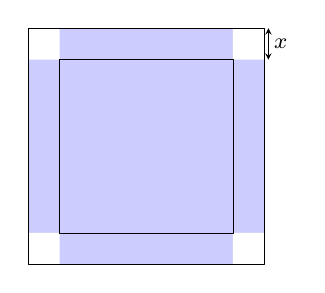
\begin{tikzpicture}[>=stealth,line join=round,line cap=round,font=\footnotesize,scale=1]
			\fill[blue!20] (0,0)--(3,0)--(3,3)--(0,3);
			\fill[white] (0,0)--(0,0.4)--(0.4,0.4)--(0.4,0) (2.6,0)--(3,0)--(3,0.4)--(2.6,0.4)
			(2.6,2.6)--(2.6,3)--(3,3)--(3,2.6) (0,2.6)--(0.4,2.6)--(0.4,3)--(0,3);
			\draw (0,0)--(3,0)--(3,3)--(0,3)--cycle;
			\draw[line width=0.2pt] (0.4,0.4)--(2.6,0.4)--(2.6,2.6)--(0.4,2.6)--cycle;
			\draw [line width=0.05pt,<->] (3.05,2.6)--(3.05,3);
			\path (3,2.6)--(3,3)node[pos=0.5,right,black]{$x$};					
		\end{tikzpicture}~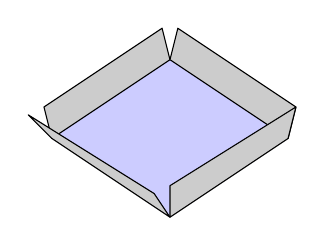
\begin{tikzpicture}[>=stealth,line join=round,line cap=round,font=\footnotesize,scale=1]
			\fill[blue!20] (0,0)--(1.5,-1)--(3,0)--(1.5,1);		
			\fill[black!20] (0,0)--(-0.1,0.4)--(1.4,1.4)--(1.5,1);
			\draw (0,0)--(-0.1,0.4)--(1.4,1.4)--(1.5,1)--cycle;
			\fill[black!20] (1.5,1)--(1.6,1.4)--(3.1,0.4)--(3,0);
			\draw (1.5,1)--(1.6,1.4)--(3.1,0.4)--(3,0)--cycle;
			\fill[black!20] (1.5,-1)--(1.5,-0.6)--(3.1,0.4)--(3,0);
			\draw (1.5,-1)--(1.5,-0.6)--(3.1,0.4)--(3,0)--cycle;
			\fill[black!20] (1.5,-1)--(1.3,-0.7)--(-0.3,0.3)--(0,0);
			\draw (1.5,-1)--(1.3,-0.7)--(-0.3,0.3)--(0,0)--cycle;
		\end{tikzpicture}
	\end{center}
	Độ dài cạnh hình vuông cần cắt bỏ để chiếc hộp đạt thể tích lớn nhất là bao nhiêu?
	\shortans{$1$}
	\loigiai{
	Mặt đáy của hộp là hình vuông có cạnh bằng $6-2x$ (cm), với $0<x<3$. Vậy diện tích của đáy hộp là $S=(6-2x)^2$.\\
	Khối hộp có chiều cao $h=x$ (cm).\\
	Vậy thể tích hộp là $V=S\cdot h=(6-2x)^2 \cdot x=4x^3-24x^2+36x$ (cm$^3$).\\
	Xét hàm $f(x)=4x^3-24x^2+36x,\,\,0<x<3$.\\
	Ta có $f'(x)=12x^2-48x+36\Rightarrow f'(x)=0\Leftrightarrow x^2-4x+3=0\Leftrightarrow \hoac{& x=1\\ & x=3.}$\\
	Ta có bảng biến thiên:
					\begin{center}
						
\begin{tikzpicture}[>=stealth]
							\tkzTabInit[nocadre=false,lgt=1.5,espcl=2,deltacl=0.5]{$x$/.7 ,$f'(x)$/.7,$f(x)$/2}
							{$0$, $1$ , $3$ }
							\tkzTabLine{ , + , $0$ , - , $0$ }
							\tkzTabVar{-/$0$ , +/$16$ , -/$0$ }
						\end{tikzpicture}
					\end{center}
	Vậy hình vuông mà bạn Việt cần cắt bỏ có độ dài cạnh $x=1$ cm thì chiếc hộp đạt thể tích lớn nhất.
	}
\end{ex}

\begin{ex}%[2D1V3-6]
	Cho một hình trụ nội tiếp trong hình nón có chiều cao bằng $12$ cm và bán kính đáy bằng $5$ cm (Hình $1$). Người ta cắt hình nón, trụ này theo mặt phẳng chứa đường thẳng nối đỉnh và tâm hình tròn đáy của hình nón thì thu được một hình phẳng như Hình $2$.
	\begin{center}
		\begin{tikzpicture}[scale=0.7, font=\footnotesize, line join=round, line cap=round, >=stealth]
			\def \x{2.5} %bán kính trục lớn elip
			\pgfmathsetmacro{\a}{\x/2};
			\def \y{0.7} %bán kính trục bé elip
			\pgfmathsetmacro{\b}{\y/2};
			\def \h{5} %chiều cao hình nón
			\coordinate (O) at (0,0);
			\coordinate (S) at ($(O)+(0,\h)$);
			\coordinate (A) at (180:\x cm and \y cm);
			\coordinate (B) at (0:\x cm and \y cm);
			\draw[dashed] (B) arc (0:180:\x cm and \y cm);
			\draw (B) arc (0:-180:\x cm and \y cm);
			\coordinate (M) at (-\a,\h/2);
			\coordinate (N) at (\a,\h/2);
			\draw[dashed] (N) arc (0:180:\a cm and \b cm);
			\draw (N) arc (0:-180:\a cm and \b cm);
			\coordinate (P) at (\a,0);
			\draw[dashed] (P) arc (0:360:\a cm and \b cm);
			\coordinate (Q) at (-\a,0);
			\draw (S)--(A) (S)--(B);
			\draw[dashed] (M)--(Q) (N)--(P);
			\node at (0,-1.5){Hình $1$};
		\end{tikzpicture}
		\qquad\qquad
		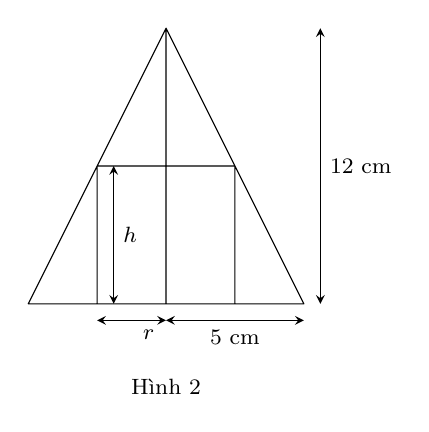
\begin{tikzpicture}[scale=0.7, font=\footnotesize, line join=round, line cap=round, >=stealth]
			\def \r{1.25} %bán kính đáy
			\def \h{2.5}
			\draw (0,2*\h)--(-2*\r,0)--(2*\r,0)--(0,2*\h)--(0,0) (-\r,0)--(-\r,\h)--(\r,\h)--(\r,0);
			\draw[<->] (-\r+0.3,0)--(-\r+0.3,\h);
			\node at (-\r+0.3,\h/2) [right]{$h$};
			\draw[<->] (-\r,-0.3)--(0,-0.3);
			\node at (-\r/4,-0.3) [below]{$r$};
			\draw[<->] (0,-0.3)--(2*\r,-0.3);
			\node at (\r,-0.3) [below]{$5$ cm};
			\draw[<->] (2*\r+0.3,0)--(2*\r+0.3,2*\h);
			\node at (2*\r+0.3,\h) [right]{$12$ cm};
			\node at (0,-1.5){Hình 2};
		\end{tikzpicture}
	\end{center}
	Tìm $h$ để khối trụ có thể tích lớn nhất.
	\shortans{$4$}
	\loigiai{
	\immini{
	Giả sử ta có hình vẽ như hình bên.\\
	Khi đó $\triangle SMN\backsim \triangle SAO$ nên
				$$\dfrac{MN}{AO}=\dfrac{SN}{SO} \Leftrightarrow \dfrac{r}{5}=\dfrac{12-h}{12}.$$
				Suy ra $r=\dfrac{5\cdot (12-h)}{12}$.
			}{
				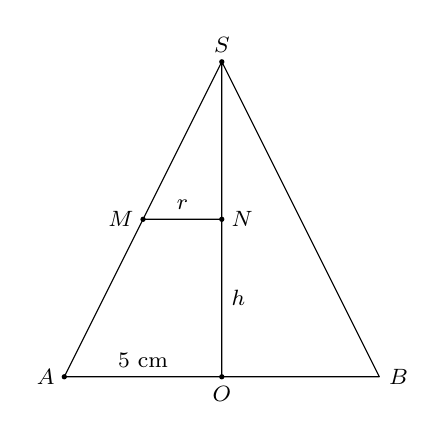
\begin{tikzpicture}[scale=.8, font=\footnotesize, line join=round, line cap=round, >=stealth]
					\def \r{1.25} %bán kính đáy
					\def \h{2.5}
					\coordinate[label=above:$S$] (S) at (0,2*\h);
					\coordinate[label=left:$A$] (A) at (-2*\r,0);
					\coordinate[label=right:$B$] (B) at (2*\r,0);
					\coordinate[label=below:$O$] (O) at (0,0);
					\coordinate[label=left:$M$] (M) at (-\r,\h);
					\coordinate[label=right:$N$] (N) at (0,\h);
					\node at (-\r/2,\h) [above]{$r$};
					\node at (0,\h/2) [right]{$h$};
					\node at (-\r,0) [above]{$5$ cm};
					\draw (S)--(A)--(B)--(S)--(O) (M)--(N);
					\foreach \diem in {S,A,O,M,N}	\fill (\diem)circle(1.2pt);
				\end{tikzpicture}
			}
	Thể tích khối trụ là
	$$V=h\pi\cdot r^2=h\pi\cdot\left(\dfrac{5\cdot (12-h)}{12}\right)^2=\dfrac{25\pi\cdot h\cdot (12-h)^2}{144}.$$
	Ta có $V(h)=\dfrac{25\pi\cdot h\cdot (12-h)^2}{144}=\dfrac{25\pi}{144}\cdot (h^3-24h^2+144h)$, với $h\in (0;12)$.
	$$\Rightarrow V'(h)=\dfrac{25\pi}{144}\cdot (3h^2-48h+144); V'(h)=0 \Leftrightarrow \hoac{& h=4\\& h=12.}$$
			Bảng biến thiên
			\begin{center}
				
\begin{tikzpicture}
					\tkzTabInit[nocadre=false,lgt=1.5,espcl=4,deltacl=0.6]
					{$h$ /0.6,$V'(h)$ /0.6,$V(h)$ /2}
					{$0$,$4$,$12$}
					\tkzTabLine{,+,$0$,-,$0$}
					\tkzTabVar{-/$0$, +/$\dfrac{400\pi}{9}$,-/$0$}
				\end{tikzpicture}
			\end{center}
			Vậy khi $h=4$ thì thể tích $V(h)$ lớn nhất.
	}
\end{ex}

\begin{ex}%[2D1V3-6]
	Một người nông dân có $15\, 000\, 000$ đồng để làm một hàng rào hình chữ E dọc theo một con sông bao quanh hai khu đất trồng rau có dạng hai hình chữ nhật bằng nhau (Hình bên dưới). Đối với mặt hàng rào song song với bờ sông thì chi phí nguyên vật liệu là $60\, 000$ đồng/mét, còn đối với ba mặt hàng rào song song với nhau thì chi phí nguyên vật liệu là $50\, 000$ đồng/mét, mặt giáp với bờ sông không phải rào. Tìm diện tích lớn nhất của hai khu đất thu được sau khi làm hàng rào.
	\begin{center}
		\begin{tikzpicture}[scale=.8, font=\footnotesize, line join=round, line cap=round, >=stealth]
			\fill[white!80!green] (-1,-.5) rectangle (12.5,2);
			\fill[white!70!cyan] (-1,2) rectangle (12.5,3);
			\fill[white!90!brown] (0,0)--(10,0)--(11.8,2)--(1.8,2)--cycle;
			
			\tikzset{tru/.pic=
				{\shade[top color=brown, bottom color=brown!50, shading angle={100}, fill=brown!70,rounded corners=0.5ex,thick]
					(0:0)--++(90:.8)--++(60:.2)--++(-60:.2)--++(-90:.8)--cycle;
					\draw[fill=black!50] (.1,.6) circle (.2mm);	}
			}
			\draw[line width=1mm,brown!50] (0,.6)--(10,.6);
			\draw[line width=1mm,brown!50] (0,0)--(10.2,0);
			\foreach \x in {0,1,2,3,...,25} {\pic at (.4*\x,0) {tru};}
			
			\tikzset{cot/.pic=
				{\shade[top color=brown, bottom color=brown!50, shading angle={100}, fill=brown!70,rounded corners=0.5ex,thick]
					(0:0)--++(90:.75)--++(60:.1)--++(-60:.1)--++(-90:.75)--cycle;}
			}
			\draw[line width=.5mm,brown!50] (0,2)--(12.5,2);
			\draw[line width=1mm,brown!50] (0,0)--(1.8,2) (0,.55)--(1.8,2.55);
			\draw[line width=1mm,brown!50] (5,0)--(6.8,2) (5,.55)--(6.8,2.55);
			\draw[line width=1mm,brown!50] (10,0)--(11.8,2) (10,.55)--(11.8,2.55);
			\foreach \x in {0,.5,1,1.5,...,5} {\pic at (.35*\x,.4*\x) {cot};}	
			\foreach \x in {0,.5,1,1.5,...,5} {\pic at ($(10,0)+(.35*\x,.4*\x)$) {cot};}
			\foreach \x in {0,.5,1,1.5,...,5} {\pic at ($(5,0)+(.35*\x,.4*\x)$) {cot};}	
			
		\end{tikzpicture}
	\end{center}
	\shortans{$6250$}
	\loigiai{
		Gọi $x \text{ (m)}$ là chiều dài của mặt hàng rào song song với bờ sông.\\
		Chi phí làm mặt hàng rào song song với bờ sông là $60000x$.\\
		Chi phí làm ba mặt hàng rào song song với nhau là $15000000-60000x$.\\
		Chiều dài của một mặt hàng rào song song với nhau là $\dfrac{15000000-60000x}{3\cdot 50000}=\left( \dfrac{-2x+500}{5}\right)$.\\	
		Diện tích của khu đất là $S(x)=x\left( \dfrac{-2x+500}{5}\right)=-\dfrac{2}{5}x^2+100x$ ($0<x<250$).\\
		Xét hàm số $f(x)= -\dfrac{2}{5}x^2+100x$ trên khoảng $(0;250)$.\\
		$f^\prime (x)=-\dfrac{4}{5}x+100$, $f^\prime (x)=0\Leftrightarrow -\dfrac{4}{5}x+100=0\Leftrightarrow x=125$.\\
		Bảng biến thiên hàm số $f(x)$ trên khoảng $(0;250)$
		\begin{center}
			
\begin{tikzpicture}
				\tkzTabInit[lgt=1.2,espcl=2.5,deltacl=0.6]
				{$x$/0.6,$f'(x)$/0.6,$f(x)$/2} {$0$,$125$,$250$}
				\tkzTabLine{,+,0,-,}
				\tkzTabVar{-/$0$,+/$6250$,-/$0$}
			\end{tikzpicture}
		\end{center}
		Từ bảng biến thiên suy ra $\max\limits_{(0;250)} f(x)=f(125)=6250$.\\
		Vậy bác nông dân có thể rào được mảnh vườn có diện tích lớn nhất $6250 \text{ m}^2$. Với chiều dài mặt hàng rào song song với bờ sông là $125 \text{ m}$ và chiều dài ba mặt song song là $50 \text{ m}$.
	}
\end{ex}

\begin{ex}%[2D1V3-6]
	Một công ty muốn làm một đường ống dẫn từ vị trí $A$ trên bờ biển đến vị trí $B$ trên hòn đảo. Khoảng cách từ điểm $B$ đến bờ biển là $BH=6$ km (Hình bên dưới). Giá tiền để xây dựng đường ống trên bờ là $50\,000$ USD mỗi kilômét và giá tiền xây dựng đường ống trên biển là $130\,000$ USD mỗi kilômét, biết rằng $AH=9$ km. Xác định vị trí điểm $C$ cách vị trí $A$ một khoảng bao nhiêu để khi lắp ống dẫn theo đường gấp khúc $ACB$ thì chi phí công ty bỏ ra là thấp nhất.
	\begin{center}
		\begin{tikzpicture}[declare function={r=12;},>=stealth]
			\foreach \i  in {0.2,0.6,...,5}
			{\draw[ultra thin,cyan,dash pattern=on 4pt off 4pt] (0,\i)--(r,\i);}
			\foreach \i   in {0,0.4,0.8,...,5}
			{\draw[ultra thin,cyan,dash pattern=on 4pt off 4pt,dash phase=4pt]
				(0,\i)--(r,\i);}
			\fill[pattern=dots,pattern color=gray!65] (0,0) rectangle (r,-1.25);
			\fill[gray!90!black] (2,4) coordinate (O) ellipse (1.65 and 1);
			\path ($(O)+(-65:1.65 and 1)$) coordinate (B)
			($(B)+(0,-1)$) coordinate (Bt)
			({0.95*r},0) coordinate (A)
			({0.5*r},0) coordinate (C)
			(intersection of B--Bt and A--C) coordinate (H);
			\draw[dashed] (B)--(H) node[pos=0.5,sloped,above,rotate=180]{$6$ km};
			\draw (B)--(C) (H)--(A);
			\path (C)--(A)--([turn]-90:0.65) coordinate (xt)
			($(H)-(A)+(xt)$) coordinate (yt);
			\draw[>=stealth,|<->|] (xt)--(yt) node[fill=white,inner sep=0pt,midway,sloped]{$9\ \mathrm{km}$};
			\foreach \t/\g in {A/-90,B/0,C/-90,H/-90}{
				\fill (\t) circle (1.5pt) node[shift={(\g:7pt)},font=\small]{$ \t $};
			}
		\end{tikzpicture}
	\end{center}
	\shortans{$6{,}5$}
	\loigiai{
		Đặt $AC=x$, với $x\in[0,9]$.
		Khi đó $BC=\sqrt{BH^2+HC^2}=\sqrt{6^2+(9-x)^2}$.\\
		Tổng chi phí công ty bỏ ra để lắp ống dẫn dẫn theo đường gấp khúc $ACB$ là
		$$
			C(x)=50 000x+130 000 \sqrt{6^2+(9-x)^2}=10000\left(5x+13\sqrt{6^2+(9-x)^2}\right).
		$$
		Do đó, chi phí công ty bỏ ra là thấp nhất khi $f(x)=5x+13\sqrt{6^2+(9-x)^2}$ đạt giá trị nhỏ nhất.\\
		Ta có $f'(x)=5+\dfrac {13(x-9)}{\sqrt {36+\left(9-x \right)^2}}$.\\
		Suy ra $f'(x)=0 \Leftrightarrow 5\sqrt {36+\left(9-x \right)^2}=13(x-9) \Leftrightarrow x=\dfrac{13}{2}\cdot$\\
		Ta có $f(0)=13\sqrt{117}$, $f\left(\dfrac{13}{2}\right)=117$ và $f(9)=123$.\\
		Từ đó, chi phí công ty bỏ ra thấp nhất khi $x=\dfrac{13}{2}=6{,}5$.\\
		Vậy với $AC=6{,}5$ khi lắp ống dẫn theo đường gấp khúc $ACB$ thì chi phí công ty bỏ ra là thấp nhất.
	}
\end{ex}

\begin{ex}%[2D1H1-5]
	Dân số của một quốc gia sau $t$ (năm) kể từ năm $2024$ được ước tính bởi công thức $N(t)=100\mathrm{e}^{0, 012t}$ ($N(t)$ được tính bằng triệu người, $0\le t\le 50$).\\
	Vào năm nào tốc độ tăng dân số của quốc gia đó là $1{,}6$ triệu người/năm?
	\shortans{$2047$}
	\loigiai{
	Trên đoạn $\left[0;50\right]$ ta có $N'(t)=0{,}012\cdot 100 \mathrm{e}^{0{,}012t}=1,2 \mathrm{e}^{0{,}012t}>0$ với mọi $t \in \left[0;50\right]$. \\ 
	Do đó, hàm số $N(t)$ đồng biến trên đoạn $\left[0;50\right]$.\\
	Ta có $N'(t)=1{,}2 \mathrm{e}^{0{,}012t}$. \\ 
	Với tốc độ tăng dân số của quốc gia đó là $1,6$ triệu người/năm ta có \\ 
	$1{,}6=1{,}2\mathrm{e}^{0{,}012t}\Leftrightarrow{\mathrm{e}^{0{,}012t}}=\dfrac{4}{3}\Leftrightarrow t=\dfrac{250\ln \dfrac{4}{3}}{3}\approx 23{,}97$. \\ 
	Vậy vào năm $2047$ thì tốc độ tăng dân số của quốc gia đó là $1{,}6$ triệu người/năm.
	}
\end{ex}

\begin{ex}%[2D1C3-6]
	Hình vẽ bên dưới mô tả đoạn đường đi vào GARA ô-tô nhà thầy Anh. Đoạn đường đầu tiên có chiều rộng bằng $x$ (m), đoạn đường thẳng vào cổng GARA có chiều rộng $2{,}6$ (m). Biết kích thước xe ô-tô là $5$m $\times$ $1{,}9$m. Để tính toán và thiết kế đường đi cho ô-tô người ta coi ô-tô như một khối hộp chữ nhật có kích thước chiều dài $5$ (m), chiều rộng $1{,}9$ (m). Hỏi chiều rộng nhỏ nhất của đoạn đường đầu tiên bằng bao nhiêu mét để ô-tô có thể đi vào GARA được? (Làm tròn kết quả đến chữ số thập phân thứ nhất)
\begin{center}
	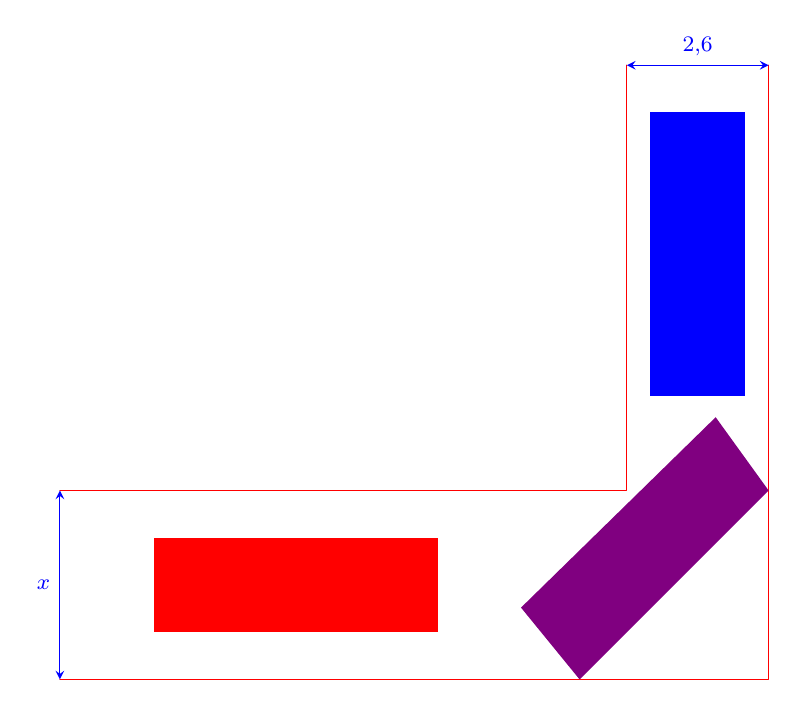
\begin{tikzpicture}[scale=.6, font=\footnotesize, line join=round, line cap=round, >=stealth]
\draw[red]	(-12,0)--(0,0)--(0,9)	(-12,-4)--(3,-4)--(3,9);
\fill[red]	(-10,-1)--(-10,-3)--(-4,-3)--(-4,-1);
\fill[violet]	(-1,-4)--(-2.24,-2.48)--(1.88,1.55)--(3,0);
\fill[blue]	(.5,2)--(2.5,2)--(2.5,8)--(.5,8);
\draw[blue,<->] 	(-12,0)--(-12,-4) node[pos=0.5,left]{$x$}; 
\draw[blue,<->] 	(0,9)--(3,9) node[pos=0.5,above]{$2{,}6$};
\end{tikzpicture}
\end{center}
	\shortans{$3{,}7$}
	\loigiai{
\begin{center}
	\begin{tikzpicture}[scale=.6, font=\footnotesize, line join=round, line cap=round, >=stealth]
		\draw[red]	(-12,0)--(0,0)--(0,9)	(-12,-4)--(3,-4);
		\draw[->,blue] (3,-4)--(3,9) node[right]{$y$};
		\draw[->,blue] (3,-4)--(6,-4) node[below]{$x$};
		\fill[blue] (3,-4) circle (1pt) node[below]{$O$};
		\draw[violet]	(-1,-4)--(-2.24,-2.48)--(1.88,1.55)--(3,0)--cycle;
		\fill[violet] (-1,-4) circle (1pt) node[below]{$B$};
		\fill[violet] (-2.24,-2.48) circle (1pt) node[left]{$C$};
		\fill[violet] (1.88,1.55) circle (1pt) node[above]{$D$};
		\fill[violet] (3,0) circle (1pt) node[right]{$A$};
		\fill[red] (0,0) circle (0pt) node[above left]{$M$};
		\fill	(1.5,-2) circle (0pt) node[below left]{$5$};
		\fill	(1.5,0) circle (0pt) node[above right]{$1{,}9$};
	\end{tikzpicture}
\end{center}
Chọn hệ trục $Oxy$ như hình vẽ. Khi đó $M(-2,6;x)$.\\
Gọi $B(-a;0)$ suy ra $A\left(0;\sqrt{25-a^2}\right)$.\\
Phương trình $AB\colon \dfrac{x}{-a}+\dfrac{y}{\sqrt{25-a^2}}-1=0$.\\
Do $CD \parallel AB$ nên phương trình $CD\colon \dfrac{x}{-a}+\dfrac{y}{\sqrt{25-a^2}}-T=0$.\\
Mà khoảng cách giữa $AB$ và $CD$ bằng $1{,}9$ nên
$$
\dfrac{|T-1|}{\sqrt{\left(\dfrac{1}{a}\right)^2+\left(\dfrac{1}{\sqrt{25-a^2}}\right)^2}}=1,9 \Rightarrow T=1+\dfrac{9,5}{a \sqrt{25-a^2}} .
$$
Điều kiện để ô-tô đi qua được là $M$, $O$ nằm khác phía đối với bờ là đường thẳng $CD$.\\
Suy ra
$$
\dfrac{-2,6}{-a}+\dfrac{x}{\sqrt{25-a^2}}-1-\dfrac{9,5}{a \sqrt{25-a^2}} \geq 0 \Leftrightarrow x \geq \sqrt{25-a^2}+\dfrac{9,5}{a}-\dfrac{2,6 \cdot \sqrt{25-a^2}}{a}.
$$
Xét hàm số $f(a)=\sqrt{25-a^2}+\dfrac{9,5}{a}-\dfrac{2,6 \cdot \sqrt{25-a^2}}{a}$ ($0<a<5$).\\
Khảo sát hàm số trên ta được giá trị lớn nhất của $f(a) \approx 3{,}7$.\\
Vậy chiều rộng nhỏ nhất của đoạn đường đầu tiên xấp xỉ $3{,}7$ m thì ô-tô có thể đi vào GARA.
	}
\end{ex}

\Closesolutionfile{ans}
\indapan{6}{ans/ans-0-B5-KQ}